\documentclass[a4paper]{book}
\usepackage{a4wide}
\usepackage{makeidx}
\usepackage{fancyhdr}
\usepackage{graphicx}
\usepackage{multicol}
\usepackage{float}
\usepackage{textcomp}
\usepackage{alltt}
\usepackage{times}
\usepackage{ifpdf}
\ifpdf
\usepackage[pdftex,
            pagebackref=true,
            colorlinks=true,
            linkcolor=blue,
            unicode
           ]{hyperref}
\else
\usepackage[ps2pdf,
            pagebackref=true,
            colorlinks=true,
            linkcolor=blue,
            unicode
           ]{hyperref}
\usepackage{pspicture}
\fi
\usepackage[utf8]{inputenc}
\usepackage{doxygen}
\makeindex
\setcounter{tocdepth}{3}
\renewcommand{\footrulewidth}{0.4pt}
\begin{document}
\begin{titlepage}
\vspace*{7cm}
\begin{center}
{\Large Reference Manual}\\
\vspace*{1cm}
{\large Generated by Doxygen 1.5.8}\\
\vspace*{0.5cm}
{\small Sat Nov 7 02:30:05 2009}\\
\end{center}
\end{titlepage}
\clearemptydoublepage
\pagenumbering{roman}
\tableofcontents
\clearemptydoublepage
\pagenumbering{arabic}
\chapter{Class Index}
\section{Class Hierarchy}
This inheritance list is sorted roughly, but not completely, alphabetically:\begin{CompactList}
\item \contentsline{section}{BaseAI::BaseAI}{\pageref{classBaseAI_1_1BaseAI}}{}
\begin{CompactList}
\item \contentsline{section}{AI::AI}{\pageref{classAI_1_1AI}}{}
\end{CompactList}
\item GameObject::GameObject\begin{CompactList}
\item \contentsline{section}{GameObject::Building}{\pageref{classGameObject_1_1Building}}{}
\item \contentsline{section}{GameObject::BuildingType}{\pageref{classGameObject_1_1BuildingType}}{}
\item \contentsline{section}{GameObject::Portal}{\pageref{classGameObject_1_1Portal}}{}
\item \contentsline{section}{GameObject::Terrain}{\pageref{classGameObject_1_1Terrain}}{}
\item \contentsline{section}{GameObject::Unit}{\pageref{classGameObject_1_1Unit}}{}
\item \contentsline{section}{GameObject::UnitType}{\pageref{classGameObject_1_1UnitType}}{}
\end{CompactList}
\end{CompactList}

\chapter{Class Index}
\section{Class List}
Here are the classes, structs, unions and interfaces with brief descriptions:\begin{CompactList}
\item\contentsline{section}{\hyperlink{classAI}{AI} (The class implementing gameplay logic )}{\pageref{classAI}}{}
\item\contentsline{section}{\hyperlink{classBaseAI}{BaseAI} (A basic \hyperlink{classAI}{AI} interface )}{\pageref{classBaseAI}}{}
\item\contentsline{section}{\hyperlink{classBuilding}{Building} (A building to shelter, feed, and/or create units )}{\pageref{classBuilding}}{}
\item\contentsline{section}{\hyperlink{classBuildingType}{BuildingType} (This defines the attributes of a kind of building )}{\pageref{classBuildingType}}{}
\item\contentsline{section}{\hyperlink{classPortal}{Portal} (A connection between two adjacent times )}{\pageref{classPortal}}{}
\item\contentsline{section}{\hyperlink{classTerrain}{Terrain} (The attributes of a specific tile of the world )}{\pageref{classTerrain}}{}
\item\contentsline{section}{\hyperlink{classUnit}{Unit} (An entitiy that can move around the game and act )}{\pageref{classUnit}}{}
\item\contentsline{section}{\hyperlink{classUnitType}{UnitType} (This defines the attributes of a kind of unit )}{\pageref{classUnitType}}{}
\end{CompactList}

\chapter{Class Documentation}
\hypertarget{classAI}{
\section{AI Class Reference}
\label{classAI}\index{AI@{AI}}
}
The class implementing gameplay logic.  


{\tt \#include $<$AI.h$>$}

Inheritance diagram for AI::\begin{figure}[H]
\begin{center}
\leavevmode
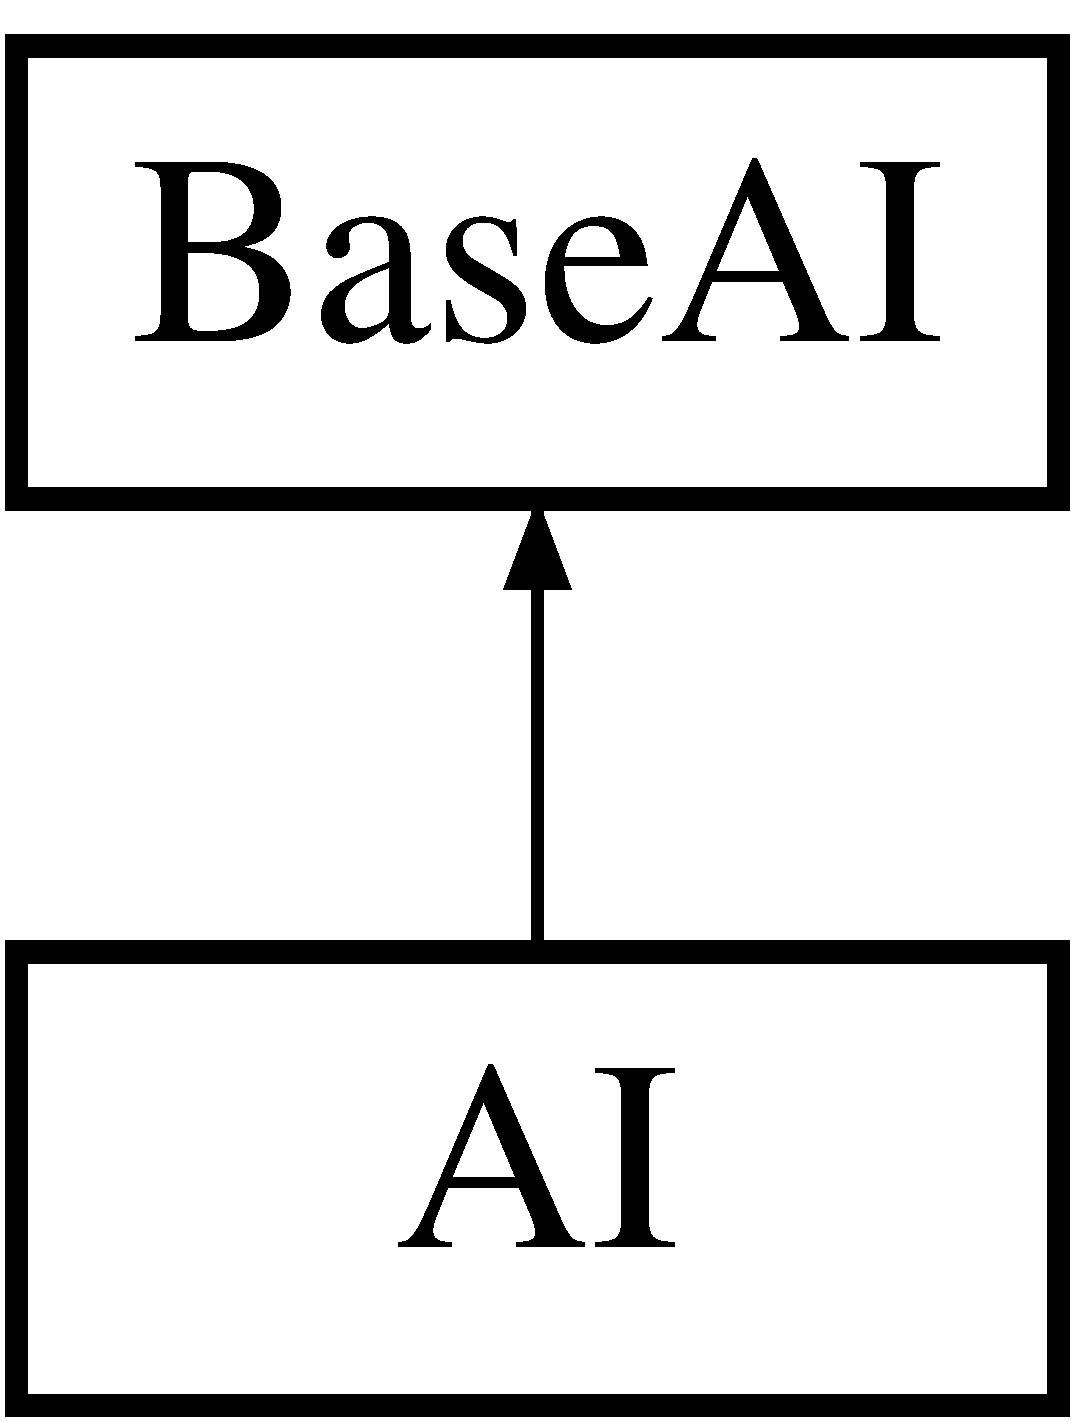
\includegraphics[height=2cm]{classAI}
\end{center}
\end{figure}
\subsection*{Public Member Functions}
\begin{CompactItemize}
\item 
virtual const char $\ast$ \hyperlink{classAI_529ac74a6f88a82abb1edd87847203e1}{username} ()
\item 
virtual const char $\ast$ \hyperlink{classAI_a4e58e11bbbdb040e6b12f8706763a00}{password} ()
\item 
virtual void \hyperlink{classAI_8c8e3a635791abaa61585357e6a25f63}{init} ()
\item 
\hypertarget{classAI_3c4746756b699cee5225597506521a39}{
virtual bool \textbf{run} ()}
\label{classAI_3c4746756b699cee5225597506521a39}

\end{CompactItemize}


\subsection{Detailed Description}
The class implementing gameplay logic. 

\subsection{Member Function Documentation}
\hypertarget{classAI_8c8e3a635791abaa61585357e6a25f63}{
\index{AI@{AI}!init@{init}}
\index{init@{init}!AI@{AI}}
\subsubsection[{init}]{\setlength{\rightskip}{0pt plus 5cm}void AI::init ()\hspace{0.3cm}{\tt  \mbox{[}virtual\mbox{]}}}}
\label{classAI_8c8e3a635791abaa61585357e6a25f63}


This is run on turn 1 before run 

Implements \hyperlink{classBaseAI_90ce8becd6f2e32c2cc32d41145e88df}{BaseAI}.\hypertarget{classAI_a4e58e11bbbdb040e6b12f8706763a00}{
\index{AI@{AI}!password@{password}}
\index{password@{password}!AI@{AI}}
\subsubsection[{password}]{\setlength{\rightskip}{0pt plus 5cm}const char $\ast$ AI::password ()\hspace{0.3cm}{\tt  \mbox{[}virtual\mbox{]}}}}
\label{classAI_a4e58e11bbbdb040e6b12f8706763a00}


Make this your password, which should be provided. 

Implements \hyperlink{classBaseAI_9251e20447917cda64ad1487b903456f}{BaseAI}.\hypertarget{classAI_529ac74a6f88a82abb1edd87847203e1}{
\index{AI@{AI}!username@{username}}
\index{username@{username}!AI@{AI}}
\subsubsection[{username}]{\setlength{\rightskip}{0pt plus 5cm}const char $\ast$ AI::username ()\hspace{0.3cm}{\tt  \mbox{[}virtual\mbox{]}}}}
\label{classAI_529ac74a6f88a82abb1edd87847203e1}


Make this your username, which should be provided. 

Implements \hyperlink{classBaseAI_ef082fbf306fec04515ed5ed3b1ba582}{BaseAI}.

The documentation for this class was generated from the following files:\begin{CompactItemize}
\item 
AI.h\item 
AI.cpp\end{CompactItemize}

\hypertarget{classBaseAI}{
\section{BaseAI Class Reference}
\label{classBaseAI}\index{BaseAI@{BaseAI}}
}
A basic \hyperlink{classAI}{AI} interface.  


Inheritance diagram for BaseAI::\begin{figure}[H]
\begin{center}
\leavevmode
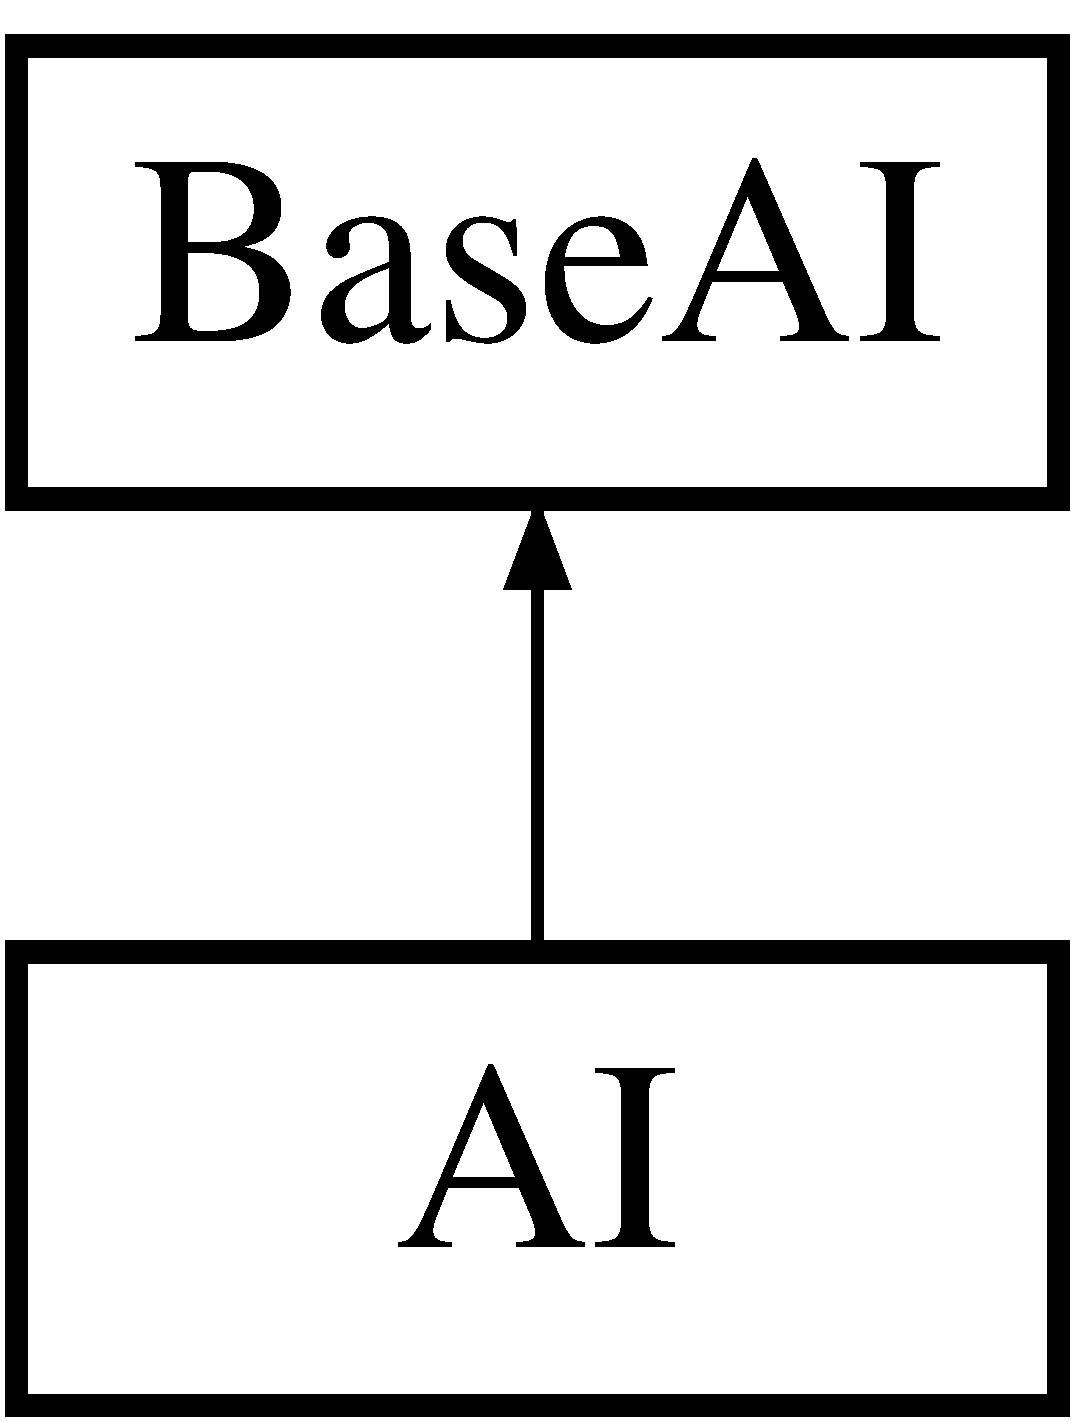
\includegraphics[height=2cm]{classBaseAI}
\end{center}
\end{figure}
\subsection*{Public Member Functions}
\begin{CompactItemize}
\item 
abstract String \hyperlink{classBaseAI_a26770dd7db8dd0c4466dd770d4e05ba}{username} ()
\item 
abstract String \hyperlink{classBaseAI_8607533e2b5bd9920ded593ae6509f48}{password} ()
\item 
abstract void \hyperlink{classBaseAI_71b49f4ca248bfd32a9f9557cb6d494a}{init} ()
\item 
abstract boolean \hyperlink{classBaseAI_56c96a58c1f1e93d17f9817711a45594}{run} ()
\item 
\hypertarget{classBaseAI_862e05b3099817fcceb55beeef7225fe}{
boolean \textbf{startTurn} ()}
\label{classBaseAI_862e05b3099817fcceb55beeef7225fe}

\end{CompactItemize}
\subsection*{Package Functions}
\begin{CompactItemize}
\item 
int \hyperlink{classBaseAI_e7574c0a95bc4431f83078c0074b1eec}{maxX} ()
\item 
int \hyperlink{classBaseAI_68f5dfd6450be2649c8c26481ba7c0a5}{maxY} ()
\item 
int \hyperlink{classBaseAI_e350c70cf7c368175a418a8fd8c29eba}{player0Gold0} ()
\item 
int \hyperlink{classBaseAI_55de649fba1edb2c8a316070a4041f16}{player0Gold1} ()
\item 
int \hyperlink{classBaseAI_5ea60d2c86f1e4457bef7963a3d0afce}{player0Gold2} ()
\item 
int \hyperlink{classBaseAI_f82cc7bd092d0636eb8a8df82a0c5b49}{player1Gold0} ()
\item 
int \hyperlink{classBaseAI_cc09926bd744fdf9ec4448366d8b8de7}{player1Gold1} ()
\item 
int \hyperlink{classBaseAI_35bad13d289478aa2bb628d6e3c56c52}{player1Gold2} ()
\item 
int \hyperlink{classBaseAI_16aab1036653c8f8fb5370cf2f6a3e10}{playerID} ()
\item 
int \hyperlink{classBaseAI_19ade7391bfe101884a35f48fb840199}{turnNumber} ()
\item 
\hyperlink{classUnitType}{UnitType} \hyperlink{classBaseAI_9bd3c6a1259db084fa6780d50bea95eb}{getTypeFromUnit} (\hyperlink{classUnit}{Unit} u)
\item 
\hyperlink{classBuildingType}{BuildingType} \hyperlink{classBaseAI_ca41bf18cdb670b9bcc5fe92eae198ad}{getTypeFromBuilding} (\hyperlink{classBuilding}{Building} b)
\item 
boolean \hyperlink{classBaseAI_2c7a4223bdc14056161c650c218369b3}{canMove} (int x, int y, int z)
\item 
boolean \hyperlink{classBaseAI_fcd72f9782c984b69f60db45756d73c4}{canBuild} (int x, int y, int z)
\item 
int \hyperlink{classBaseAI_0643622ad827a6ad035bf84dfdfacd55}{effDamage} (\hyperlink{classUnitType}{UnitType} ut, int level)
\item 
int \hyperlink{classBaseAI_ec102e33572b1f58df437260bf73141e}{effFood} (\hyperlink{classBuildingType}{BuildingType} bt, int level)
\item 
int \hyperlink{classBaseAI_c079405ee4fd5cec789af0f627d3d175}{getGold} (int playerNum, int z)
\item 
int \hyperlink{classBaseAI_9a6e10da16c3b209915251ca183815e7}{artWorth} (int artistLevel, int galleryLevel)
\item 
int \hyperlink{classBaseAI_e1677c15b8b022dd7335eeb84b57b30f}{hunger} (int playerID, int z)
\item 
int \hyperlink{classBaseAI_43314f174d849c294ec84a09af6b55e2}{foodProduced} (int playerID, int z)
\item 
int \hyperlink{classBaseAI_d49ab218e79412c1ce975159688e6cfd}{effBuildingPrice} (\hyperlink{classBuildingType}{BuildingType} bt, int level)
\item 
int \hyperlink{classBaseAI_5995a3d005840158948db900a312092c}{effUnitPrice} (\hyperlink{classBuildingType}{BuildingType} bt, int level)
\item 
int \hyperlink{classBaseAI_0977f4ba22e8b97f89d7b0c03941c788}{effUnitMaxHP} (\hyperlink{classUnitType}{UnitType} ut, int level)
\item 
int \hyperlink{classBaseAI_2f6a6c6f1da75c203de7e1b1abe7bed1}{effBuildingMaxHP} (\hyperlink{classBuildingType}{BuildingType} bt, int level)
\item 
int \hyperlink{classBaseAI_1de8bdc9274ca62632b9fb7caf55800e}{effBuildingArmor} (\hyperlink{classBuildingType}{BuildingType} bt, int level)
\item 
int \hyperlink{classBaseAI_b08916c060ca84af1c0ba12e8ec9d54c}{effUnitArmor} (\hyperlink{classUnitType}{UnitType} ut, int level)
\end{CompactItemize}
\subsection*{Package Attributes}
\begin{CompactItemize}
\item 
\hypertarget{classBaseAI_94966bbfdac0d091a7332f19b29935c3}{
boolean \textbf{initialized}}
\label{classBaseAI_94966bbfdac0d091a7332f19b29935c3}

\end{CompactItemize}
\subsection*{Static Package Attributes}
\begin{CompactItemize}
\item 
\hypertarget{classBaseAI_926e4ea0d21e83c40c866aca231f9bfb}{
static \hyperlink{classBuilding}{Building}\mbox{[}$\,$\mbox{]} \textbf{buildings}}
\label{classBaseAI_926e4ea0d21e83c40c866aca231f9bfb}

\item 
\hypertarget{classBaseAI_89467168401b45cac54330db953c3127}{
static \hyperlink{classBuildingType}{BuildingType}\mbox{[}$\,$\mbox{]} \textbf{buildingTypes}}
\label{classBaseAI_89467168401b45cac54330db953c3127}

\item 
\hypertarget{classBaseAI_e916f205bfd024dc0ed704a382e72af9}{
static \hyperlink{classPortal}{Portal}\mbox{[}$\,$\mbox{]} \textbf{portals}}
\label{classBaseAI_e916f205bfd024dc0ed704a382e72af9}

\item 
\hypertarget{classBaseAI_6c6bf690012338f0284e2ec6ac85d4e2}{
static \hyperlink{classTerrain}{Terrain}\mbox{[}$\,$\mbox{]} \textbf{terrains}}
\label{classBaseAI_6c6bf690012338f0284e2ec6ac85d4e2}

\item 
\hypertarget{classBaseAI_72140772daaa7cd0a0fdab17cabc5b87}{
static \hyperlink{classUnit}{Unit}\mbox{[}$\,$\mbox{]} \textbf{units}}
\label{classBaseAI_72140772daaa7cd0a0fdab17cabc5b87}

\item 
\hypertarget{classBaseAI_db07b81437b69901c160762cbfb9dfd0}{
static \hyperlink{classUnitType}{UnitType}\mbox{[}$\,$\mbox{]} \textbf{unitTypes}}
\label{classBaseAI_db07b81437b69901c160762cbfb9dfd0}

\item 
\hypertarget{classBaseAI_d7942cee117a347f7cb841ff4800408f}{
static int \textbf{iteration}}
\label{classBaseAI_d7942cee117a347f7cb841ff4800408f}

\end{CompactItemize}


\subsection{Detailed Description}
A basic \hyperlink{classAI}{AI} interface. 

This class implements most the code an \hyperlink{classAI}{AI} would need to interface with the lower-level game code. AIs should extend this class to get a lot of builer-plate code out of the way The provided \hyperlink{classAI}{AI} class does just that. 

\subsection{Member Function Documentation}
\hypertarget{classBaseAI_9a6e10da16c3b209915251ca183815e7}{
\index{BaseAI@{BaseAI}!artWorth@{artWorth}}
\index{artWorth@{artWorth}!BaseAI@{BaseAI}}
\subsubsection[{artWorth}]{\setlength{\rightskip}{0pt plus 5cm}int BaseAI::artWorth (int {\em artistLevel}, \/  int {\em galleryLevel})\hspace{0.3cm}{\tt  \mbox{[}inline, package\mbox{]}}}}
\label{classBaseAI_9a6e10da16c3b209915251ca183815e7}


Returns the amount of gold that would be gained if an artist at the given level paints at a gallery of the given level. \hypertarget{classBaseAI_fcd72f9782c984b69f60db45756d73c4}{
\index{BaseAI@{BaseAI}!canBuild@{canBuild}}
\index{canBuild@{canBuild}!BaseAI@{BaseAI}}
\subsubsection[{canBuild}]{\setlength{\rightskip}{0pt plus 5cm}boolean BaseAI::canBuild (int {\em x}, \/  int {\em y}, \/  int {\em z})\hspace{0.3cm}{\tt  \mbox{[}inline, package\mbox{]}}}}
\label{classBaseAI_fcd72f9782c984b69f60db45756d73c4}


Returns true if this square is clear for you to build on.

This function checks to see if this square contains any enemy units, buildings, or blocking terrain. This is not an efficient implementation. Feel free to write your own. \hypertarget{classBaseAI_2c7a4223bdc14056161c650c218369b3}{
\index{BaseAI@{BaseAI}!canMove@{canMove}}
\index{canMove@{canMove}!BaseAI@{BaseAI}}
\subsubsection[{canMove}]{\setlength{\rightskip}{0pt plus 5cm}boolean BaseAI::canMove (int {\em x}, \/  int {\em y}, \/  int {\em z})\hspace{0.3cm}{\tt  \mbox{[}inline, package\mbox{]}}}}
\label{classBaseAI_2c7a4223bdc14056161c650c218369b3}


Returns true if one of your units could move to the given coordinate

This function checks to see if this square contains any enemy units, enemy buildings, or blocking terrain. This is not an efficient implementation. Feel free to write your own. \hypertarget{classBaseAI_1de8bdc9274ca62632b9fb7caf55800e}{
\index{BaseAI@{BaseAI}!effBuildingArmor@{effBuildingArmor}}
\index{effBuildingArmor@{effBuildingArmor}!BaseAI@{BaseAI}}
\subsubsection[{effBuildingArmor}]{\setlength{\rightskip}{0pt plus 5cm}int BaseAI::effBuildingArmor ({\bf BuildingType} {\em bt}, \/  int {\em level})\hspace{0.3cm}{\tt  \mbox{[}inline, package\mbox{]}}}}
\label{classBaseAI_1de8bdc9274ca62632b9fb7caf55800e}


Returns the armor of a building of the given type and level. \hypertarget{classBaseAI_2f6a6c6f1da75c203de7e1b1abe7bed1}{
\index{BaseAI@{BaseAI}!effBuildingMaxHP@{effBuildingMaxHP}}
\index{effBuildingMaxHP@{effBuildingMaxHP}!BaseAI@{BaseAI}}
\subsubsection[{effBuildingMaxHP}]{\setlength{\rightskip}{0pt plus 5cm}int BaseAI::effBuildingMaxHP ({\bf BuildingType} {\em bt}, \/  int {\em level})\hspace{0.3cm}{\tt  \mbox{[}inline, package\mbox{]}}}}
\label{classBaseAI_2f6a6c6f1da75c203de7e1b1abe7bed1}


Returns the maxHP of a building of the given type and level. \hypertarget{classBaseAI_d49ab218e79412c1ce975159688e6cfd}{
\index{BaseAI@{BaseAI}!effBuildingPrice@{effBuildingPrice}}
\index{effBuildingPrice@{effBuildingPrice}!BaseAI@{BaseAI}}
\subsubsection[{effBuildingPrice}]{\setlength{\rightskip}{0pt plus 5cm}int BaseAI::effBuildingPrice ({\bf BuildingType} {\em bt}, \/  int {\em level})\hspace{0.3cm}{\tt  \mbox{[}inline, package\mbox{]}}}}
\label{classBaseAI_d49ab218e79412c1ce975159688e6cfd}


Returns the price of a building of the given type and level. \hypertarget{classBaseAI_0643622ad827a6ad035bf84dfdfacd55}{
\index{BaseAI@{BaseAI}!effDamage@{effDamage}}
\index{effDamage@{effDamage}!BaseAI@{BaseAI}}
\subsubsection[{effDamage}]{\setlength{\rightskip}{0pt plus 5cm}int BaseAI::effDamage ({\bf UnitType} {\em ut}, \/  int {\em level})\hspace{0.3cm}{\tt  \mbox{[}inline, package\mbox{]}}}}
\label{classBaseAI_0643622ad827a6ad035bf84dfdfacd55}


Returns the amount of raw damage a given type of unit would cause at the given level. \hypertarget{classBaseAI_ec102e33572b1f58df437260bf73141e}{
\index{BaseAI@{BaseAI}!effFood@{effFood}}
\index{effFood@{effFood}!BaseAI@{BaseAI}}
\subsubsection[{effFood}]{\setlength{\rightskip}{0pt plus 5cm}int BaseAI::effFood ({\bf BuildingType} {\em bt}, \/  int {\em level})\hspace{0.3cm}{\tt  \mbox{[}inline, package\mbox{]}}}}
\label{classBaseAI_ec102e33572b1f58df437260bf73141e}


Returns the amount of food produced by a given type of building at the given level. \hypertarget{classBaseAI_b08916c060ca84af1c0ba12e8ec9d54c}{
\index{BaseAI@{BaseAI}!effUnitArmor@{effUnitArmor}}
\index{effUnitArmor@{effUnitArmor}!BaseAI@{BaseAI}}
\subsubsection[{effUnitArmor}]{\setlength{\rightskip}{0pt plus 5cm}int BaseAI::effUnitArmor ({\bf UnitType} {\em ut}, \/  int {\em level})\hspace{0.3cm}{\tt  \mbox{[}inline, package\mbox{]}}}}
\label{classBaseAI_b08916c060ca84af1c0ba12e8ec9d54c}


Returns the armor of a unit of the given type and level. \hypertarget{classBaseAI_0977f4ba22e8b97f89d7b0c03941c788}{
\index{BaseAI@{BaseAI}!effUnitMaxHP@{effUnitMaxHP}}
\index{effUnitMaxHP@{effUnitMaxHP}!BaseAI@{BaseAI}}
\subsubsection[{effUnitMaxHP}]{\setlength{\rightskip}{0pt plus 5cm}int BaseAI::effUnitMaxHP ({\bf UnitType} {\em ut}, \/  int {\em level})\hspace{0.3cm}{\tt  \mbox{[}inline, package\mbox{]}}}}
\label{classBaseAI_0977f4ba22e8b97f89d7b0c03941c788}


Returns the maxHP of a building of the given type and level. \hypertarget{classBaseAI_5995a3d005840158948db900a312092c}{
\index{BaseAI@{BaseAI}!effUnitPrice@{effUnitPrice}}
\index{effUnitPrice@{effUnitPrice}!BaseAI@{BaseAI}}
\subsubsection[{effUnitPrice}]{\setlength{\rightskip}{0pt plus 5cm}int BaseAI::effUnitPrice ({\bf BuildingType} {\em bt}, \/  int {\em level})\hspace{0.3cm}{\tt  \mbox{[}inline, package\mbox{]}}}}
\label{classBaseAI_5995a3d005840158948db900a312092c}


Returns the price of a unit of the given type and level. \hypertarget{classBaseAI_43314f174d849c294ec84a09af6b55e2}{
\index{BaseAI@{BaseAI}!foodProduced@{foodProduced}}
\index{foodProduced@{foodProduced}!BaseAI@{BaseAI}}
\subsubsection[{foodProduced}]{\setlength{\rightskip}{0pt plus 5cm}int BaseAI::foodProduced (int {\em playerID}, \/  int {\em z})\hspace{0.3cm}{\tt  \mbox{[}inline, package\mbox{]}}}}
\label{classBaseAI_43314f174d849c294ec84a09af6b55e2}


Returns the sum of all food produced by all buildings owned by the given player in the given time period. \hypertarget{classBaseAI_c079405ee4fd5cec789af0f627d3d175}{
\index{BaseAI@{BaseAI}!getGold@{getGold}}
\index{getGold@{getGold}!BaseAI@{BaseAI}}
\subsubsection[{getGold}]{\setlength{\rightskip}{0pt plus 5cm}int BaseAI::getGold (int {\em playerNum}, \/  int {\em z})\hspace{0.3cm}{\tt  \mbox{[}inline, package\mbox{]}}}}
\label{classBaseAI_c079405ee4fd5cec789af0f627d3d175}


Returns the amount of gold the given player has in the given time period \hypertarget{classBaseAI_ca41bf18cdb670b9bcc5fe92eae198ad}{
\index{BaseAI@{BaseAI}!getTypeFromBuilding@{getTypeFromBuilding}}
\index{getTypeFromBuilding@{getTypeFromBuilding}!BaseAI@{BaseAI}}
\subsubsection[{getTypeFromBuilding}]{\setlength{\rightskip}{0pt plus 5cm}{\bf BuildingType} BaseAI::getTypeFromBuilding ({\bf Building} {\em b})\hspace{0.3cm}{\tt  \mbox{[}inline, package\mbox{]}}}}
\label{classBaseAI_ca41bf18cdb670b9bcc5fe92eae198ad}


Returns the type of the given building. \hypertarget{classBaseAI_9bd3c6a1259db084fa6780d50bea95eb}{
\index{BaseAI@{BaseAI}!getTypeFromUnit@{getTypeFromUnit}}
\index{getTypeFromUnit@{getTypeFromUnit}!BaseAI@{BaseAI}}
\subsubsection[{getTypeFromUnit}]{\setlength{\rightskip}{0pt plus 5cm}{\bf UnitType} BaseAI::getTypeFromUnit ({\bf Unit} {\em u})\hspace{0.3cm}{\tt  \mbox{[}inline, package\mbox{]}}}}
\label{classBaseAI_9bd3c6a1259db084fa6780d50bea95eb}


Returns the type of the given unit. \hypertarget{classBaseAI_e1677c15b8b022dd7335eeb84b57b30f}{
\index{BaseAI@{BaseAI}!hunger@{hunger}}
\index{hunger@{hunger}!BaseAI@{BaseAI}}
\subsubsection[{hunger}]{\setlength{\rightskip}{0pt plus 5cm}int BaseAI::hunger (int {\em playerID}, \/  int {\em z})\hspace{0.3cm}{\tt  \mbox{[}inline, package\mbox{]}}}}
\label{classBaseAI_e1677c15b8b022dd7335eeb84b57b30f}


Returns the sum of all hunger values for all units owned by the given player in the given time period. \hypertarget{classBaseAI_71b49f4ca248bfd32a9f9557cb6d494a}{
\index{BaseAI@{BaseAI}!init@{init}}
\index{init@{init}!BaseAI@{BaseAI}}
\subsubsection[{init}]{\setlength{\rightskip}{0pt plus 5cm}abstract void BaseAI::init ()\hspace{0.3cm}{\tt  \mbox{[}pure virtual\mbox{]}}}}
\label{classBaseAI_71b49f4ca248bfd32a9f9557cb6d494a}


This is run on turn 1 before run 

Implemented in \hyperlink{classAI_8c8e3a635791abaa61585357e6a25f63}{AI}.\hypertarget{classBaseAI_e7574c0a95bc4431f83078c0074b1eec}{
\index{BaseAI@{BaseAI}!maxX@{maxX}}
\index{maxX@{maxX}!BaseAI@{BaseAI}}
\subsubsection[{maxX}]{\setlength{\rightskip}{0pt plus 5cm}int BaseAI::maxX ()\hspace{0.3cm}{\tt  \mbox{[}inline, package\mbox{]}}}}
\label{classBaseAI_e7574c0a95bc4431f83078c0074b1eec}


Gets the X boundary for the map in all time periods.

For each time period, the map is a rectangle from (-max\_\-x,-max\_\-y) to (max\_\-x,max\_\-y) \hypertarget{classBaseAI_68f5dfd6450be2649c8c26481ba7c0a5}{
\index{BaseAI@{BaseAI}!maxY@{maxY}}
\index{maxY@{maxY}!BaseAI@{BaseAI}}
\subsubsection[{maxY}]{\setlength{\rightskip}{0pt plus 5cm}int BaseAI::maxY ()\hspace{0.3cm}{\tt  \mbox{[}inline, package\mbox{]}}}}
\label{classBaseAI_68f5dfd6450be2649c8c26481ba7c0a5}


Gets the Y boundary for the map in all time periods.

For each time period, the map is a rectangle from (-max\_\-x,-max\_\-y) to (max\_\-x,max\_\-y) \hypertarget{classBaseAI_8607533e2b5bd9920ded593ae6509f48}{
\index{BaseAI@{BaseAI}!password@{password}}
\index{password@{password}!BaseAI@{BaseAI}}
\subsubsection[{password}]{\setlength{\rightskip}{0pt plus 5cm}abstract String BaseAI::password ()\hspace{0.3cm}{\tt  \mbox{[}pure virtual\mbox{]}}}}
\label{classBaseAI_8607533e2b5bd9920ded593ae6509f48}


Make this your password, which should be provided. 

Implemented in \hyperlink{classAI_405047fd39e03de993183392a06d655b}{AI}.\hypertarget{classBaseAI_e350c70cf7c368175a418a8fd8c29eba}{
\index{BaseAI@{BaseAI}!player0Gold0@{player0Gold0}}
\index{player0Gold0@{player0Gold0}!BaseAI@{BaseAI}}
\subsubsection[{player0Gold0}]{\setlength{\rightskip}{0pt plus 5cm}int BaseAI::player0Gold0 ()\hspace{0.3cm}{\tt  \mbox{[}inline, package\mbox{]}}}}
\label{classBaseAI_e350c70cf7c368175a418a8fd8c29eba}


Returns the amount of gold player 0 has in the far past Also see int \hyperlink{classBaseAI_c079405ee4fd5cec789af0f627d3d175}{BaseAI::getGold(int playerNum, int z)} \hypertarget{classBaseAI_55de649fba1edb2c8a316070a4041f16}{
\index{BaseAI@{BaseAI}!player0Gold1@{player0Gold1}}
\index{player0Gold1@{player0Gold1}!BaseAI@{BaseAI}}
\subsubsection[{player0Gold1}]{\setlength{\rightskip}{0pt plus 5cm}int BaseAI::player0Gold1 ()\hspace{0.3cm}{\tt  \mbox{[}inline, package\mbox{]}}}}
\label{classBaseAI_55de649fba1edb2c8a316070a4041f16}


Returns the amount of gold player 0 has in the past Also see int \hyperlink{classBaseAI_c079405ee4fd5cec789af0f627d3d175}{BaseAI::getGold(int playerNum, int z)} \hypertarget{classBaseAI_5ea60d2c86f1e4457bef7963a3d0afce}{
\index{BaseAI@{BaseAI}!player0Gold2@{player0Gold2}}
\index{player0Gold2@{player0Gold2}!BaseAI@{BaseAI}}
\subsubsection[{player0Gold2}]{\setlength{\rightskip}{0pt plus 5cm}int BaseAI::player0Gold2 ()\hspace{0.3cm}{\tt  \mbox{[}inline, package\mbox{]}}}}
\label{classBaseAI_5ea60d2c86f1e4457bef7963a3d0afce}


Returns the amount of gold player 0 has in the present Also see int \hyperlink{classBaseAI_c079405ee4fd5cec789af0f627d3d175}{BaseAI::getGold(int playerNum, int z)} \hypertarget{classBaseAI_f82cc7bd092d0636eb8a8df82a0c5b49}{
\index{BaseAI@{BaseAI}!player1Gold0@{player1Gold0}}
\index{player1Gold0@{player1Gold0}!BaseAI@{BaseAI}}
\subsubsection[{player1Gold0}]{\setlength{\rightskip}{0pt plus 5cm}int BaseAI::player1Gold0 ()\hspace{0.3cm}{\tt  \mbox{[}inline, package\mbox{]}}}}
\label{classBaseAI_f82cc7bd092d0636eb8a8df82a0c5b49}


Returns the amount of gold player 1 has in the far past Also see int \hyperlink{classBaseAI_c079405ee4fd5cec789af0f627d3d175}{BaseAI::getGold(int playerNum, int z)} \hypertarget{classBaseAI_cc09926bd744fdf9ec4448366d8b8de7}{
\index{BaseAI@{BaseAI}!player1Gold1@{player1Gold1}}
\index{player1Gold1@{player1Gold1}!BaseAI@{BaseAI}}
\subsubsection[{player1Gold1}]{\setlength{\rightskip}{0pt plus 5cm}int BaseAI::player1Gold1 ()\hspace{0.3cm}{\tt  \mbox{[}inline, package\mbox{]}}}}
\label{classBaseAI_cc09926bd744fdf9ec4448366d8b8de7}


Returns the amount of gold player 1 has in the past Also see int \hyperlink{classBaseAI_c079405ee4fd5cec789af0f627d3d175}{BaseAI::getGold(int playerNum, int z)} \hypertarget{classBaseAI_35bad13d289478aa2bb628d6e3c56c52}{
\index{BaseAI@{BaseAI}!player1Gold2@{player1Gold2}}
\index{player1Gold2@{player1Gold2}!BaseAI@{BaseAI}}
\subsubsection[{player1Gold2}]{\setlength{\rightskip}{0pt plus 5cm}int BaseAI::player1Gold2 ()\hspace{0.3cm}{\tt  \mbox{[}inline, package\mbox{]}}}}
\label{classBaseAI_35bad13d289478aa2bb628d6e3c56c52}


Returns the amount of gold player 1 has in the present Also see int \hyperlink{classBaseAI_c079405ee4fd5cec789af0f627d3d175}{BaseAI::getGold(int playerNum, int z)} \hypertarget{classBaseAI_16aab1036653c8f8fb5370cf2f6a3e10}{
\index{BaseAI@{BaseAI}!playerID@{playerID}}
\index{playerID@{playerID}!BaseAI@{BaseAI}}
\subsubsection[{playerID}]{\setlength{\rightskip}{0pt plus 5cm}int BaseAI::playerID ()\hspace{0.3cm}{\tt  \mbox{[}inline, package\mbox{]}}}}
\label{classBaseAI_16aab1036653c8f8fb5370cf2f6a3e10}


Returns the your player ID, either 0 or 1.

This value will match the ownerID of all your units. \hypertarget{classBaseAI_56c96a58c1f1e93d17f9817711a45594}{
\index{BaseAI@{BaseAI}!run@{run}}
\index{run@{run}!BaseAI@{BaseAI}}
\subsubsection[{run}]{\setlength{\rightskip}{0pt plus 5cm}abstract boolean BaseAI::run ()\hspace{0.3cm}{\tt  \mbox{[}pure virtual\mbox{]}}}}
\label{classBaseAI_56c96a58c1f1e93d17f9817711a45594}


This is run every turn . Return true to end the turn, return false to request a status update from the server and then immediately rerun this function with the latest game status. 

Implemented in \hyperlink{classAI_f25b3a076daef2aaf9f74ecf458bdfbc}{AI}.\hypertarget{classBaseAI_19ade7391bfe101884a35f48fb840199}{
\index{BaseAI@{BaseAI}!turnNumber@{turnNumber}}
\index{turnNumber@{turnNumber}!BaseAI@{BaseAI}}
\subsubsection[{turnNumber}]{\setlength{\rightskip}{0pt plus 5cm}int BaseAI::turnNumber ()\hspace{0.3cm}{\tt  \mbox{[}inline, package\mbox{]}}}}
\label{classBaseAI_19ade7391bfe101884a35f48fb840199}


Returns the current turn number

The first turn is turn 0. Player 0 gets the first turn. The second turn is turn 1. Player 1 gets the first turn. The game is ends at the end of turn 499 or earlier. \hypertarget{classBaseAI_a26770dd7db8dd0c4466dd770d4e05ba}{
\index{BaseAI@{BaseAI}!username@{username}}
\index{username@{username}!BaseAI@{BaseAI}}
\subsubsection[{username}]{\setlength{\rightskip}{0pt plus 5cm}abstract String BaseAI::username ()\hspace{0.3cm}{\tt  \mbox{[}pure virtual\mbox{]}}}}
\label{classBaseAI_a26770dd7db8dd0c4466dd770d4e05ba}


Make this your username, which should be provided. 

Implemented in \hyperlink{classAI_d7e6db6b414a192ad2af8656d012cfdc}{AI}.

The documentation for this class was generated from the following file:\begin{CompactItemize}
\item 
BaseAI.java\end{CompactItemize}

\hypertarget{classBuilding}{
\section{Building Class Reference}
\label{classBuilding}\index{Building@{Building}}
}
A building to shelter, feed, and/or create units.  


\subsection*{Public Member Functions}
\begin{CompactItemize}
\item 
\hypertarget{classBuilding_5bb038e1c890d73c2161ff08ea6086a0}{
\textbf{Building} (Pointer p)}
\label{classBuilding_5bb038e1c890d73c2161ff08ea6086a0}

\item 
\hypertarget{classBuilding_f7bea63fbc209c3a348720eabda2625d}{
int \textbf{getObjectID} ()}
\label{classBuilding_f7bea63fbc209c3a348720eabda2625d}

\item 
\hypertarget{classBuilding_028fed33d87eb61bbfe964937e887349}{
int \textbf{getX} ()}
\label{classBuilding_028fed33d87eb61bbfe964937e887349}

\item 
\hypertarget{classBuilding_675148df2cf1596be3c60b9935751847}{
int \textbf{getY} ()}
\label{classBuilding_675148df2cf1596be3c60b9935751847}

\item 
\hypertarget{classBuilding_df2b7cb86eba3958df598c112a71b824}{
int \textbf{getZ} ()}
\label{classBuilding_df2b7cb86eba3958df598c112a71b824}

\item 
\hypertarget{classBuilding_941600423b8f67aeb5b5fb7eae40c259}{
int \textbf{getHp} ()}
\label{classBuilding_941600423b8f67aeb5b5fb7eae40c259}

\item 
\hypertarget{classBuilding_caaed1f1d99a7cc94c8466c68851f6a7}{
int \textbf{getLevel} ()}
\label{classBuilding_caaed1f1d99a7cc94c8466c68851f6a7}

\item 
\hypertarget{classBuilding_d78120c8f3447bc9738d300e0d82468e}{
int \textbf{getBuildingTypeID} ()}
\label{classBuilding_d78120c8f3447bc9738d300e0d82468e}

\item 
\hypertarget{classBuilding_853c197c784ea28355d1801c60ea0ece}{
int \textbf{getOwnerID} ()}
\label{classBuilding_853c197c784ea28355d1801c60ea0ece}

\item 
\hypertarget{classBuilding_86e78c67cbc3218550b175c2a8954845}{
int \textbf{getInTraining} ()}
\label{classBuilding_86e78c67cbc3218550b175c2a8954845}

\item 
\hypertarget{classBuilding_5ce7ab40f4138247a799a197dddc5209}{
int \textbf{getProgress} ()}
\label{classBuilding_5ce7ab40f4138247a799a197dddc5209}

\item 
\hypertarget{classBuilding_8c97bfce86d3678c45999a620f4c0d96}{
int \textbf{getLinked} ()}
\label{classBuilding_8c97bfce86d3678c45999a620f4c0d96}

\item 
\hypertarget{classBuilding_e99952041bb8b3832609a46252406989}{
int \textbf{getComplete} ()}
\label{classBuilding_e99952041bb8b3832609a46252406989}

\end{CompactItemize}
\subsection*{Package Functions}
\begin{CompactItemize}
\item 
\hypertarget{classBuilding_07d6cee891a31ea6314763ce416e774f}{
boolean \textbf{validify} ()}
\label{classBuilding_07d6cee891a31ea6314763ce416e774f}

\item 
\hypertarget{classBuilding_dd956b0c3891f6f7a708d03f360ea78d}{
boolean \textbf{train} (\hyperlink{classUnitType}{UnitType} unit)}
\label{classBuilding_dd956b0c3891f6f7a708d03f360ea78d}

\item 
\hypertarget{classBuilding_e445fb3ceb3b359a9bbfffdf7f1982ab}{
boolean \textbf{cancel} ()}
\label{classBuilding_e445fb3ceb3b359a9bbfffdf7f1982ab}

\end{CompactItemize}
\subsection*{Package Attributes}
\begin{CompactItemize}
\item 
\hypertarget{classBuilding_57899d00333919397552519ef8299fd6}{
Pointer \textbf{ptr}}
\label{classBuilding_57899d00333919397552519ef8299fd6}

\item 
\hypertarget{classBuilding_44b3e8718773800e0d7fb464b19012b3}{
int \textbf{ID}}
\label{classBuilding_44b3e8718773800e0d7fb464b19012b3}

\item 
\hypertarget{classBuilding_28cb3992ff16427fbe5d84c61939d433}{
int \textbf{iteration}}
\label{classBuilding_28cb3992ff16427fbe5d84c61939d433}

\end{CompactItemize}


\subsection{Detailed Description}
A building to shelter, feed, and/or create units. 

The documentation for this class was generated from the following file:\begin{CompactItemize}
\item 
Building.java\end{CompactItemize}

\hypertarget{classBuildingType}{
\section{BuildingType Class Reference}
\label{classBuildingType}\index{BuildingType@{BuildingType}}
}
This defines the attributes of a kind of building.  


{\tt \#include $<$wrappers.h$>$}

\subsection*{Public Member Functions}
\begin{CompactItemize}
\item 
\hypertarget{classBuildingType_4f4b34cfe4ee8e45f0e65f6c5d4e7bb9}{
\textbf{BuildingType} (\_\-BuildingType $\ast$ptr=NULL)}
\label{classBuildingType_4f4b34cfe4ee8e45f0e65f6c5d4e7bb9}

\item 
\hypertarget{classBuildingType_e2e3b4a71736772db226889edeede525}{
int \textbf{objectID} ()}
\label{classBuildingType_e2e3b4a71736772db226889edeede525}

\item 
\hypertarget{classBuildingType_14b04f6191efd64754733064cc71c39f}{
char $\ast$ \textbf{name} ()}
\label{classBuildingType_14b04f6191efd64754733064cc71c39f}

\item 
\hypertarget{classBuildingType_56adb396d8a4a08af404261964250048}{
int \textbf{price} ()}
\label{classBuildingType_56adb396d8a4a08af404261964250048}

\item 
\hypertarget{classBuildingType_b619bcf2b8101453d041aaa3a518fbd9}{
int \textbf{food} ()}
\label{classBuildingType_b619bcf2b8101453d041aaa3a518fbd9}

\item 
\hypertarget{classBuildingType_2c41c74ad0d129c0c041d1b1d4eee23f}{
int \textbf{pastBuildTime} ()}
\label{classBuildingType_2c41c74ad0d129c0c041d1b1d4eee23f}

\item 
\hypertarget{classBuildingType_28124b76e664f95241113f2763b8465a}{
int \textbf{presentBuildTime} ()}
\label{classBuildingType_28124b76e664f95241113f2763b8465a}

\item 
\hypertarget{classBuildingType_2be0cff4241c3db8131ddabb1af105ef}{
int \textbf{futureBuildTime} ()}
\label{classBuildingType_2be0cff4241c3db8131ddabb1af105ef}

\item 
\hypertarget{classBuildingType_0782b2e15502434e037a3ab568cda60a}{
int \textbf{hp} ()}
\label{classBuildingType_0782b2e15502434e037a3ab568cda60a}

\item 
\hypertarget{classBuildingType_58e99303826f46d4cf1aa15d554f196c}{
int \textbf{armor} ()}
\label{classBuildingType_58e99303826f46d4cf1aa15d554f196c}

\item 
int \hyperlink{classBuildingType_2345e1ed48eef3ece1fab1a49a5d156c}{builderID} ()
\item 
int \hyperlink{classBuildingType_dd762a4123302708815b67c11b8029df}{allowPaint} ()
\item 
\hypertarget{classBuildingType_06da51d3d6a345f5e69f7c845a6f60e6}{
int \textbf{width} ()}
\label{classBuildingType_06da51d3d6a345f5e69f7c845a6f60e6}

\item 
\hypertarget{classBuildingType_f4dced7299e2e310f6f1ed4650b599ee}{
int \textbf{height} ()}
\label{classBuildingType_f4dced7299e2e310f6f1ed4650b599ee}

\item 
int \hyperlink{classBuildingType_af7eafec053a2235e0bd59867735cb38}{spawnX} ()
\item 
int \hyperlink{classBuildingType_2eb4a10f9714a1947b33354a7eb59d5d}{spawnY} ()
\item 
\hypertarget{classBuildingType_ac4e7a40274f1384fbb6bed347817dc3}{
float \textbf{armorExp} ()}
\label{classBuildingType_ac4e7a40274f1384fbb6bed347817dc3}

\item 
\hypertarget{classBuildingType_6ff19209c80c182f0f1efcdfc5832f77}{
float \textbf{hpExp} ()}
\label{classBuildingType_6ff19209c80c182f0f1efcdfc5832f77}

\item 
\hypertarget{classBuildingType_7680b2d1f0fe070e47c7a0e0637437d1}{
float \textbf{priceExp} ()}
\label{classBuildingType_7680b2d1f0fe070e47c7a0e0637437d1}

\item 
\hypertarget{classBuildingType_c3f36af02351f9a2f020bbf31c787518}{
float \textbf{foodExp} ()}
\label{classBuildingType_c3f36af02351f9a2f020bbf31c787518}

\end{CompactItemize}
\subsection*{Public Attributes}
\begin{CompactItemize}
\item 
\hypertarget{classBuildingType_f3ec5eaf1c1ccfdc72250183dbaa38e3}{
\_\-BuildingType $\ast$ \textbf{ptr}}
\label{classBuildingType_f3ec5eaf1c1ccfdc72250183dbaa38e3}

\end{CompactItemize}
\subsection*{Friends}
\begin{CompactItemize}
\item 
\hypertarget{classBuildingType_677ea2327738bed33cc14a91c911a4c1}{
std::ostream \& \textbf{operator$<$$<$} (std::ostream \&stream, \hyperlink{classBuildingType}{BuildingType} ob)}
\label{classBuildingType_677ea2327738bed33cc14a91c911a4c1}

\end{CompactItemize}


\subsection{Detailed Description}
This defines the attributes of a kind of building. 

\subsection{Member Function Documentation}
\hypertarget{classBuildingType_dd762a4123302708815b67c11b8029df}{
\index{BuildingType@{BuildingType}!allowPaint@{allowPaint}}
\index{allowPaint@{allowPaint}!BuildingType@{BuildingType}}
\subsubsection[{allowPaint}]{\setlength{\rightskip}{0pt plus 5cm}int BuildingType::allowPaint ()}}
\label{classBuildingType_dd762a4123302708815b67c11b8029df}


Returns 1 if this building type allows units to paint, 0 otherwise. \hypertarget{classBuildingType_2345e1ed48eef3ece1fab1a49a5d156c}{
\index{BuildingType@{BuildingType}!builderID@{builderID}}
\index{builderID@{builderID}!BuildingType@{BuildingType}}
\subsubsection[{builderID}]{\setlength{\rightskip}{0pt plus 5cm}int BuildingType::builderID ()}}
\label{classBuildingType_2345e1ed48eef3ece1fab1a49a5d156c}


Returns the object id of the unit type that can build this building type. \hypertarget{classBuildingType_af7eafec053a2235e0bd59867735cb38}{
\index{BuildingType@{BuildingType}!spawnX@{spawnX}}
\index{spawnX@{spawnX}!BuildingType@{BuildingType}}
\subsubsection[{spawnX}]{\setlength{\rightskip}{0pt plus 5cm}int BuildingType::spawnX ()}}
\label{classBuildingType_af7eafec053a2235e0bd59867735cb38}


Returns the x offest of newly created units from this building.

Newly trained units appear at (x+spawnX, y+spawnY \hypertarget{classBuildingType_2eb4a10f9714a1947b33354a7eb59d5d}{
\index{BuildingType@{BuildingType}!spawnY@{spawnY}}
\index{spawnY@{spawnY}!BuildingType@{BuildingType}}
\subsubsection[{spawnY}]{\setlength{\rightskip}{0pt plus 5cm}int BuildingType::spawnY ()}}
\label{classBuildingType_2eb4a10f9714a1947b33354a7eb59d5d}


Returns the y offest of newly created units from this building.

Newly trained units appear at (x+spawnX, y+spawnY 

The documentation for this class was generated from the following files:\begin{CompactItemize}
\item 
wrappers.h\item 
wrappers.cpp\end{CompactItemize}

\hypertarget{classPortal}{
\section{Portal Class Reference}
\label{classPortal}\index{Portal@{Portal}}
}
A connection between two adjacent times.  


\subsection*{Public Member Functions}
\begin{CompactItemize}
\item 
\hypertarget{classPortal_8a2fffc0a245d244ee1cf6eb65107f9e}{
\textbf{Portal} (Pointer p)}
\label{classPortal_8a2fffc0a245d244ee1cf6eb65107f9e}

\item 
\hypertarget{classPortal_0d9df749602425a10f502ea98e3cbf4d}{
int \textbf{getObjectID} ()}
\label{classPortal_0d9df749602425a10f502ea98e3cbf4d}

\item 
\hypertarget{classPortal_fe44ea5cfb6974808bc6fbf88d68f1cb}{
int \textbf{getX} ()}
\label{classPortal_fe44ea5cfb6974808bc6fbf88d68f1cb}

\item 
\hypertarget{classPortal_9749e055cf67bdb4a2fa997d699159ca}{
int \textbf{getY} ()}
\label{classPortal_9749e055cf67bdb4a2fa997d699159ca}

\item 
\hypertarget{classPortal_93d3e9605a606799ad5a87e39d11b980}{
int \textbf{getZ} ()}
\label{classPortal_93d3e9605a606799ad5a87e39d11b980}

\item 
\hypertarget{classPortal_2e5b1b9179301f214059b9c3e55ad422}{
int \textbf{getDirection} ()}
\label{classPortal_2e5b1b9179301f214059b9c3e55ad422}

\item 
\hypertarget{classPortal_865eb443eed6e1c82f5743092d54c488}{
int \textbf{getFee} ()}
\label{classPortal_865eb443eed6e1c82f5743092d54c488}

\item 
\hypertarget{classPortal_77a19a4968e415556805a1076eaab7c4}{
int \textbf{getFeeIncr} ()}
\label{classPortal_77a19a4968e415556805a1076eaab7c4}

\item 
\hypertarget{classPortal_2da131e32757e31d9d9e101c0a5b870d}{
float \textbf{getFeeMultiplier} ()}
\label{classPortal_2da131e32757e31d9d9e101c0a5b870d}

\end{CompactItemize}
\subsection*{Package Functions}
\begin{CompactItemize}
\item 
\hypertarget{classPortal_0de12fecec65b2e2d873bc5b612fa41b}{
boolean \textbf{validify} ()}
\label{classPortal_0de12fecec65b2e2d873bc5b612fa41b}

\end{CompactItemize}
\subsection*{Package Attributes}
\begin{CompactItemize}
\item 
\hypertarget{classPortal_085779842017d4b8c53021d29493df44}{
Pointer \textbf{ptr}}
\label{classPortal_085779842017d4b8c53021d29493df44}

\item 
\hypertarget{classPortal_afffd0cb7ff19b0abeb3dfb4919c1387}{
int \textbf{ID}}
\label{classPortal_afffd0cb7ff19b0abeb3dfb4919c1387}

\item 
\hypertarget{classPortal_8d5c901b3e23cd2775a7eef6a6babc29}{
int \textbf{iteration}}
\label{classPortal_8d5c901b3e23cd2775a7eef6a6babc29}

\end{CompactItemize}


\subsection{Detailed Description}
A connection between two adjacent times. 

The documentation for this class was generated from the following file:\begin{CompactItemize}
\item 
Portal.java\end{CompactItemize}

\hypertarget{classTerrain}{
\section{Terrain Class Reference}
\label{classTerrain}\index{Terrain@{Terrain}}
}
The attributes of a specific tile of the world.  


{\tt \#include $<$wrappers.h$>$}

\subsection*{Public Member Functions}
\begin{CompactItemize}
\item 
\hypertarget{classTerrain_d69f12c1a91d0c3b96d3e5d3006dcef9}{
\textbf{Terrain} (\_\-Terrain $\ast$ptr=NULL)}
\label{classTerrain_d69f12c1a91d0c3b96d3e5d3006dcef9}

\item 
\hypertarget{classTerrain_34577a3c0632bb51515aab9b363a65f1}{
int \textbf{objectID} ()}
\label{classTerrain_34577a3c0632bb51515aab9b363a65f1}

\item 
\hypertarget{classTerrain_ed3254c223a45d3e0f319fcc54add79a}{
int \textbf{x} ()}
\label{classTerrain_ed3254c223a45d3e0f319fcc54add79a}

\item 
\hypertarget{classTerrain_9a4db29382d784d64f6817eb738d9d4c}{
int \textbf{y} ()}
\label{classTerrain_9a4db29382d784d64f6817eb738d9d4c}

\item 
\hypertarget{classTerrain_06173b6758d8adbc82181db2a6306a75}{
int \textbf{z} ()}
\label{classTerrain_06173b6758d8adbc82181db2a6306a75}

\item 
int \hyperlink{classTerrain_80105933c1d08553db9d7c9abca47251}{blocksMove} ()
\item 
int \hyperlink{classTerrain_f2ae042e3aecc89c7746c04e2498e45b}{blocksBuild} ()
\end{CompactItemize}
\subsection*{Public Attributes}
\begin{CompactItemize}
\item 
\hypertarget{classTerrain_8f795aee94e17dc84f3cb22ca877cda9}{
\_\-Terrain $\ast$ \textbf{ptr}}
\label{classTerrain_8f795aee94e17dc84f3cb22ca877cda9}

\end{CompactItemize}
\subsection*{Friends}
\begin{CompactItemize}
\item 
\hypertarget{classTerrain_276298433a740eda4ee02befa9155ff4}{
std::ostream \& \textbf{operator$<$$<$} (std::ostream \&stream, \hyperlink{classTerrain}{Terrain} ob)}
\label{classTerrain_276298433a740eda4ee02befa9155ff4}

\end{CompactItemize}


\subsection{Detailed Description}
The attributes of a specific tile of the world. 

\subsection{Member Function Documentation}
\hypertarget{classTerrain_f2ae042e3aecc89c7746c04e2498e45b}{
\index{Terrain@{Terrain}!blocksBuild@{blocksBuild}}
\index{blocksBuild@{blocksBuild}!Terrain@{Terrain}}
\subsubsection[{blocksBuild}]{\setlength{\rightskip}{0pt plus 5cm}int Terrain::blocksBuild ()}}
\label{classTerrain_f2ae042e3aecc89c7746c04e2498e45b}


Returns 1 if this object pervents buildings from being placed on this square, 0 otherwise. \hypertarget{classTerrain_80105933c1d08553db9d7c9abca47251}{
\index{Terrain@{Terrain}!blocksMove@{blocksMove}}
\index{blocksMove@{blocksMove}!Terrain@{Terrain}}
\subsubsection[{blocksMove}]{\setlength{\rightskip}{0pt plus 5cm}int Terrain::blocksMove ()}}
\label{classTerrain_80105933c1d08553db9d7c9abca47251}


Returns 1 if this object prevents units from moving onto this square, 0 otherwise. 

The documentation for this class was generated from the following files:\begin{CompactItemize}
\item 
wrappers.h\item 
wrappers.cpp\end{CompactItemize}

\hypertarget{classUnit}{
\section{Unit Class Reference}
\label{classUnit}\index{Unit@{Unit}}
}
An entitiy that can move around the game and act.  


{\tt \#include $<$wrappers.h$>$}

\subsection*{Public Member Functions}
\begin{CompactItemize}
\item 
\hypertarget{classUnit_137b06047ff3c863b7b8b11d6166b23b}{
\textbf{Unit} (\_\-Unit $\ast$ptr=NULL)}
\label{classUnit_137b06047ff3c863b7b8b11d6166b23b}

\item 
\hypertarget{classUnit_621a32dd222ff61ae2b449929f4ca8ec}{
int \textbf{objectID} ()}
\label{classUnit_621a32dd222ff61ae2b449929f4ca8ec}

\item 
\hypertarget{classUnit_eaaab5b23cb47ac5a73b765e23d822eb}{
int \textbf{x} ()}
\label{classUnit_eaaab5b23cb47ac5a73b765e23d822eb}

\item 
\hypertarget{classUnit_ed8851f757a1d06dc12a36714436cf5d}{
int \textbf{y} ()}
\label{classUnit_ed8851f757a1d06dc12a36714436cf5d}

\item 
\hypertarget{classUnit_c0c37e2f02206836aee89d79f26c7444}{
int \textbf{z} ()}
\label{classUnit_c0c37e2f02206836aee89d79f26c7444}

\item 
\hypertarget{classUnit_b64b87b4b5111ccbc2891515148fa5b8}{
int \textbf{hp} ()}
\label{classUnit_b64b87b4b5111ccbc2891515148fa5b8}

\item 
\hypertarget{classUnit_72c9eaba718ba5f4116bd273d38d8522}{
int \textbf{level} ()}
\label{classUnit_72c9eaba718ba5f4116bd273d38d8522}

\item 
\hypertarget{classUnit_ca492d37ca3c44ce203e497d571f59d4}{
int \textbf{unitTypeID} ()}
\label{classUnit_ca492d37ca3c44ce203e497d571f59d4}

\item 
\hypertarget{classUnit_95a85f91e1969c5340765de82c203625}{
int \textbf{ownerID} ()}
\label{classUnit_95a85f91e1969c5340765de82c203625}

\item 
\hypertarget{classUnit_21d1e0167e8fd7d5ec8fceebe817df98}{
int \textbf{actions} ()}
\label{classUnit_21d1e0167e8fd7d5ec8fceebe817df98}

\item 
\hypertarget{classUnit_803f4023d9d00c501d9a0b55ac5d5126}{
int \textbf{moves} ()}
\label{classUnit_803f4023d9d00c501d9a0b55ac5d5126}

\item 
\hypertarget{classUnit_b86073c935bec5d959159d837cd9b9c3}{
bool \textbf{attack} (int x, int y)}
\label{classUnit_b86073c935bec5d959159d837cd9b9c3}

\item 
\hypertarget{classUnit_aad323acdd0a291f7d309ac24e01ab9f}{
bool \textbf{build} (int x, int y, \hyperlink{classBuildingType}{BuildingType} \&type)}
\label{classUnit_aad323acdd0a291f7d309ac24e01ab9f}

\item 
bool \hyperlink{classUnit_766eec7dc93515b6d6590fd2c12923a6}{paint} (int x, int y)
\item 
\hypertarget{classUnit_01181b403f885cc2ea06389074626e83}{
bool \textbf{move} (int x, int y)}
\label{classUnit_01181b403f885cc2ea06389074626e83}

\item 
bool \hyperlink{classUnit_46e83270573c33637b588b87132c8905}{warp} ()
\end{CompactItemize}
\subsection*{Public Attributes}
\begin{CompactItemize}
\item 
\hypertarget{classUnit_f5240a8811a31044b1170278d66412f2}{
\_\-Unit $\ast$ \textbf{ptr}}
\label{classUnit_f5240a8811a31044b1170278d66412f2}

\end{CompactItemize}
\subsection*{Friends}
\begin{CompactItemize}
\item 
\hypertarget{classUnit_bba2ea3d62724066fa08ec7d9de7833a}{
std::ostream \& \textbf{operator$<$$<$} (std::ostream \&stream, \hyperlink{classUnit}{Unit} ob)}
\label{classUnit_bba2ea3d62724066fa08ec7d9de7833a}

\end{CompactItemize}


\subsection{Detailed Description}
An entitiy that can move around the game and act. 

\subsection{Member Function Documentation}
\hypertarget{classUnit_766eec7dc93515b6d6590fd2c12923a6}{
\index{Unit@{Unit}!paint@{paint}}
\index{paint@{paint}!Unit@{Unit}}
\subsubsection[{paint}]{\setlength{\rightskip}{0pt plus 5cm}bool Unit::paint (int {\em x}, \/  int {\em y})}}
\label{classUnit_766eec7dc93515b6d6590fd2c12923a6}


The unit attempts to generate gold by painting. The x,y coordinate must contain a Gallery amd must be adjacent or under this unit. \hypertarget{classUnit_46e83270573c33637b588b87132c8905}{
\index{Unit@{Unit}!warp@{warp}}
\index{warp@{warp}!Unit@{Unit}}
\subsubsection[{warp}]{\setlength{\rightskip}{0pt plus 5cm}bool Unit::warp ()}}
\label{classUnit_46e83270573c33637b588b87132c8905}


Makes this unit attempt to use a portal.

The portal under this unit adds its direction member variable to this unit's z coordinate. The portal's fee is paid and then increased. 

The documentation for this class was generated from the following files:\begin{CompactItemize}
\item 
wrappers.h\item 
wrappers.cpp\end{CompactItemize}

\hypertarget{classUnitType}{
\section{UnitType Class Reference}
\label{classUnitType}\index{UnitType@{UnitType}}
}
This defines the attributes of a kind of unit.  


{\tt \#include $<$wrappers.h$>$}

\subsection*{Public Member Functions}
\begin{CompactItemize}
\item 
\hypertarget{classUnitType_416de534d56d49a3019fa9b2601d10f9}{
\textbf{UnitType} (\_\-UnitType $\ast$ptr=NULL)}
\label{classUnitType_416de534d56d49a3019fa9b2601d10f9}

\item 
\hypertarget{classUnitType_a153f6427546ef11334b64e44e49740a}{
int \textbf{objectID} ()}
\label{classUnitType_a153f6427546ef11334b64e44e49740a}

\item 
\hypertarget{classUnitType_3908d7cf5e0b5a2cb60b8516225e7c59}{
char $\ast$ \textbf{name} ()}
\label{classUnitType_3908d7cf5e0b5a2cb60b8516225e7c59}

\item 
\hypertarget{classUnitType_09f8d620a03f63bf063935df712c9f57}{
int \textbf{price} ()}
\label{classUnitType_09f8d620a03f63bf063935df712c9f57}

\item 
\hypertarget{classUnitType_2981e06eb4d6537fb8ca775ea20033c9}{
int \textbf{hunger} ()}
\label{classUnitType_2981e06eb4d6537fb8ca775ea20033c9}

\item 
\hypertarget{classUnitType_f8f27eea3e3c5284ba1509164c75ed96}{
int \textbf{trainTime} ()}
\label{classUnitType_f8f27eea3e3c5284ba1509164c75ed96}

\item 
\hypertarget{classUnitType_310873153e2b3c8aed99ca087974b59c}{
int \textbf{hp} ()}
\label{classUnitType_310873153e2b3c8aed99ca087974b59c}

\item 
\hypertarget{classUnitType_0f50024671abefed34ccc2636c73025c}{
int \textbf{armor} ()}
\label{classUnitType_0f50024671abefed34ccc2636c73025c}

\item 
\hypertarget{classUnitType_71686e035dcd8cfaf8eecaed61692502}{
int \textbf{moves} ()}
\label{classUnitType_71686e035dcd8cfaf8eecaed61692502}

\item 
\hypertarget{classUnitType_9026a31cea4a0c092706eb2e8bc96196}{
int \textbf{actions} ()}
\label{classUnitType_9026a31cea4a0c092706eb2e8bc96196}

\item 
\hypertarget{classUnitType_ef6755e0c8ffc6d7208c05d6b813eba6}{
int \textbf{attackCost} ()}
\label{classUnitType_ef6755e0c8ffc6d7208c05d6b813eba6}

\item 
\hypertarget{classUnitType_2e1880b083c5f41afe20f65ef9f54291}{
int \textbf{damage} ()}
\label{classUnitType_2e1880b083c5f41afe20f65ef9f54291}

\item 
\hypertarget{classUnitType_54ad12f62bb28f44ac868bd8e14d2b1c}{
int \textbf{minRange} ()}
\label{classUnitType_54ad12f62bb28f44ac868bd8e14d2b1c}

\item 
\hypertarget{classUnitType_e1607c3f741a2325b85c2975c28aa019}{
int \textbf{maxRange} ()}
\label{classUnitType_e1607c3f741a2325b85c2975c28aa019}

\item 
int \hyperlink{classUnitType_0526f93cb8c905235fd90d0d54c92bf1}{trainerID} ()
\item 
int \hyperlink{classUnitType_8be8091a55003a0901f30d7600e2d0a6}{canPaint} ()
\item 
\hypertarget{classUnitType_4fb7e90ddc386e594a7259c28ff98e28}{
float \textbf{armorExp} ()}
\label{classUnitType_4fb7e90ddc386e594a7259c28ff98e28}

\item 
\hypertarget{classUnitType_3416ec9ad9f56dd3f78cd326cc384888}{
float \textbf{hpExp} ()}
\label{classUnitType_3416ec9ad9f56dd3f78cd326cc384888}

\item 
\hypertarget{classUnitType_459679be756b33fcb912d15bb20f2cad}{
float \textbf{priceExp} ()}
\label{classUnitType_459679be756b33fcb912d15bb20f2cad}

\item 
\hypertarget{classUnitType_4adad226c65b9e3f9db1d1e8acc98892}{
float \textbf{damageExp} ()}
\label{classUnitType_4adad226c65b9e3f9db1d1e8acc98892}

\item 
\hypertarget{classUnitType_ad49a4a8e68b4c4be09c1558d0c08322}{
int \textbf{paintBase} ()}
\label{classUnitType_ad49a4a8e68b4c4be09c1558d0c08322}

\item 
\hypertarget{classUnitType_8b69461267020f890cf36aa1f276033f}{
int \textbf{paintLinear} ()}
\label{classUnitType_8b69461267020f890cf36aa1f276033f}

\end{CompactItemize}
\subsection*{Public Attributes}
\begin{CompactItemize}
\item 
\hypertarget{classUnitType_42bb83a6d9ad668ce229e4ee19e7ce0b}{
\_\-UnitType $\ast$ \textbf{ptr}}
\label{classUnitType_42bb83a6d9ad668ce229e4ee19e7ce0b}

\end{CompactItemize}
\subsection*{Friends}
\begin{CompactItemize}
\item 
\hypertarget{classUnitType_741d0ed0451b24d98ac791f3f25ad6cd}{
std::ostream \& \textbf{operator$<$$<$} (std::ostream \&stream, \hyperlink{classUnitType}{UnitType} ob)}
\label{classUnitType_741d0ed0451b24d98ac791f3f25ad6cd}

\end{CompactItemize}


\subsection{Detailed Description}
This defines the attributes of a kind of unit. 

\subsection{Member Function Documentation}
\hypertarget{classUnitType_8be8091a55003a0901f30d7600e2d0a6}{
\index{UnitType@{UnitType}!canPaint@{canPaint}}
\index{canPaint@{canPaint}!UnitType@{UnitType}}
\subsubsection[{canPaint}]{\setlength{\rightskip}{0pt plus 5cm}int UnitType::canPaint ()}}
\label{classUnitType_8be8091a55003a0901f30d7600e2d0a6}


Returns 1 if this unit can perform the paint action, 0 otherwise. \hypertarget{classUnitType_0526f93cb8c905235fd90d0d54c92bf1}{
\index{UnitType@{UnitType}!trainerID@{trainerID}}
\index{trainerID@{trainerID}!UnitType@{UnitType}}
\subsubsection[{trainerID}]{\setlength{\rightskip}{0pt plus 5cm}int UnitType::trainerID ()}}
\label{classUnitType_0526f93cb8c905235fd90d0d54c92bf1}


Returns the objectID of the building that can train this unit. 

The documentation for this class was generated from the following files:\begin{CompactItemize}
\item 
wrappers.h\item 
wrappers.cpp\end{CompactItemize}

\printindex
\end{document}
